\section{Selected regions}
\label{sec:regions}

\tab{regions} lists the regions selected from the parent volume for resimulation.

\begin{table*}
	\centering
	\caption{Regions selected from the parent volume for resimulation.
	We provide their positions within the parent volume, their overdensity $\delta$ as defined by \eq{1}, their \textit{rms} overdensity $\sigma$, and weights, $f_j$, calculated as per \sec{method:weighting}
	}
	\label{tab:regions}
	\begin{tabular}{lcccc} % four columns, alignment for each
		\hline
		index & (x, y, z)/(\cMpch) & $\delta$ & $\sigma$ & $f_j$\\
		\hline
		0 &   (623.48, 1142.15, 1525.28)  &  0.970 &  5.623 &  0.000032 \\
		1 &   (524.09, 1203.60, 1138.54)  &  0.918 &  5.406 &  0.000207 \\
		2 &   (54.22, 1709.61, 571.08)    &  0.852 &  5.117 &  0.000466 \\
		3 &   (153.61, 1762.02, 531.32)   &  0.849 &  5.106 &  0.001024 \\
		4 &   (39.76, 1686.12, 1850.57)   &  0.846 &  5.089 &  0.000494 \\
		5 &   (847.58, 1443.95, 1062.63)  &  0.842 &  5.074 &  0.000896 \\
		6 &   (1198.17, 135.54, 1375.28)  &  0.841 &  5.070 &  0.000706 \\
		7 &   (1012.03, 1514.43, 1454.80) &  0.839 &  5.062 &  0.001219 \\
		8 &   (590.95, 359.63, 1610.21)   &  0.839 &  5.059 &  0.000297 \\
		9 &   (746.37, 820.47, 945.16)    &  0.833 &  5.032 &  0.001087 \\
		10 &  (1181.91, 1171.06, 974.08)  &  0.830 &  5.022 &  0.000425 \\
		11 &  (37.95, 670.47, 46.99)      &  0.829 &  5.017 &  0.000754 \\
		12 &  (1989.73, 368.67, 2076.47)  &  0.828 &  5.010 &  0.000695 \\
		13 &  (1659.01, 1306.60, 760.83)  &  0.824 &  4.993 &  0.000528 \\
		14 &  (57.83, 883.72, 2098.16)    &  0.821 &  4.981 &  0.001280 \\
		15 &  (609.03, 2018.64, 115.66)   &  0.820 &  4.977 &  0.000807 \\
		16 &  (122.89, 1124.08, 1304.80)  &  0.616 &  4.000 &  0.003899 \\
		17 &  (1395.16, 415.66, 1575.88)  &  0.616 &  3.999 &  0.004833 \\
		18 &  (128.31, 216.86, 258.43)    &  0.431 &  3.000 &  0.009591 \\
		19 &  (1400.58, 1686.12, 806.01)  &  0.431 &  3.000 &  0.012793 \\
		20 &  (699.39, 1760.21, 1725.88)  &  0.266 &  2.000 &  0.029495 \\
		21 &  (1951.78, 2022.26, 1709.61) &  0.266 &  2.000 &  0.028335 \\
		22 &  (755.41, 1122.27, 867.46)   &  0.121 &  1.000 &  0.057656 \\
		23 &  (516.86, 325.30, 603.60)    &  0.121 &  1.000 &  0.061536 \\
		24 &  (937.94, 1382.51, 1077.09)  & -0.007 &  0.000 &  0.074118 \\
		25 &  (1675.27, 1492.75, 1335.52) & -0.007 &  0.000 &  0.079869 \\
		26 &  (1270.46, 518.67, 862.03)   & -0.121 & -1.000 &  0.063350 \\
		27 &  (242.16, 1881.30, 1624.67)  & -0.121 & -1.000 &  0.058147 \\
		28 &  (1454.80, 1720.45, 1608.41) & -0.222 & -2.000 &  0.034742 \\
		29 &  (430.11, 296.38, 359.63)    & -0.222 & -2.000 &  0.024672 \\
		30 &  (1733.10, 1096.97, 1060.83) & -0.311 & -3.000 &  0.012474 \\
		31 &  (1821.66, 946.97, 1431.30)  & -0.311 & -3.000 &  0.013408 \\
		32 &  (1913.82, 1033.72, 45.18)   & -0.066 & -0.499 &  0.063999 \\
		33 &  (2009.61, 2024.06, 1693.35) & -0.066 & -0.500 &  0.065877 \\
		34 &  (339.75, 934.32, 1646.36)   & -0.007 &  0.000 &  0.075462 \\
		35 &  (1693.35, 914.44, 1977.08)  & -0.007 & -0.000 &  0.076093 \\
		36 &  (778.90, 899.98, 1866.84)   &  0.055 &  0.501 &  0.070135 \\
		37 &  (1790.94, 1239.74, 1765.63) &  0.055 &  0.500 &  0.062186 \\
		38 &  (2078.28, 77.71, 140.96)    & -0.479 & -5.285 &  0.002858 \\
		39 &  (818.66, 110.24, 1628.29)   & -0.434 & -4.606 &  0.003555 \\
		\hline
	\end{tabular}
\end{table*}


\section{Fitted distribution functions}
\tab{schechter_params} and \ref{tab:sfrf_schechter_params} show double-Schechter fit parameters to the GSMF and SFRF.
We use \textsf{FitDF}, a python module for fitting arbitrary distribution functions using Markov Chain Monte Carlo (MCMC).
\textsf{FitDF} is built around the popular \textsf{emcee} package \citep[v3.0,][]{foreman-mackey_emcee_2013}.
The code can be found at \url{https://github.com/flaresimulations/fitDF}.

A Poisson form of the likelihood is typically used for distribution function analyses in Astronomy due to the relatively small number of observations.
Due to our resimulation approach we cannot use this form of the likelihood, since the number counts obtained from the composite approach, scaled to the size of the parent box volume, significantly underestimate the errors.
Instead, we use a Gaussian form for the likelihood,
\begin{align}
\mathrm{log}(\mathcal{L}) = - \frac{1}{2} \, \left[ \sum_{i} \, \frac{ (N_{i,\mathrm{obs}} - N_{i,\mathrm{exp}})^2 }{\sigma_{i}^{2}} \, + \mathrm{log}(\sigma_{i}^{2}) \right]
\end{align}
where the subscript $i$ represents the bin of the property being measured, $N_{i,\mathrm{obs}}$ is the inferred number of galaxies using the composite number density multiplied by the parent box volume, $N_{i,\mathrm{exp}}$ is the expected number from the model, and $\sigma_i$ is the error estimate.
Using this form, $\sigma$ can be explicitly provided from the resimulated number counts, $\sigma_{i} = N_{i,\mathrm{obs}} / \sqrt{n_{i,\mathrm{obs}}}$, where $n_{i,\mathrm{obs}}$ is the number counts in bin $i$ from the resimulations.

We use flat uniform priors in $\mathrm{log_{10}}(D^*)$, $\alpha_1$, $\mathrm{log_{10}}(\phi^*_1)$ and $\mathrm{log_{10}}(\phi^*_2)$.
We fix $\alpha_2 = -1$ by setting a narrow top-hat prior around this value.
We run chains of length $10^{4}$, then calculate the autocorrelation time, $\tau$, on these chains \citep{goodman_ensemble_2010}.
We use $\tau$ to estimate the burn-in ($\tau \times 4$) and thinning ($\tau / 2$) on our chains.
The chains for each fit are available at \url{https://flaresimulations.github.io/flares/data.html}.
Example posteriors for each parameter in a fit to the $z = 7$ GSMF are shown as a corner plot in \fig{posteriors}.

\tab{sfs_params} shows the piecewise-fits to the SFS; the fitting procedure is described in \sec{results:sfs}.

\begin{figure*}
	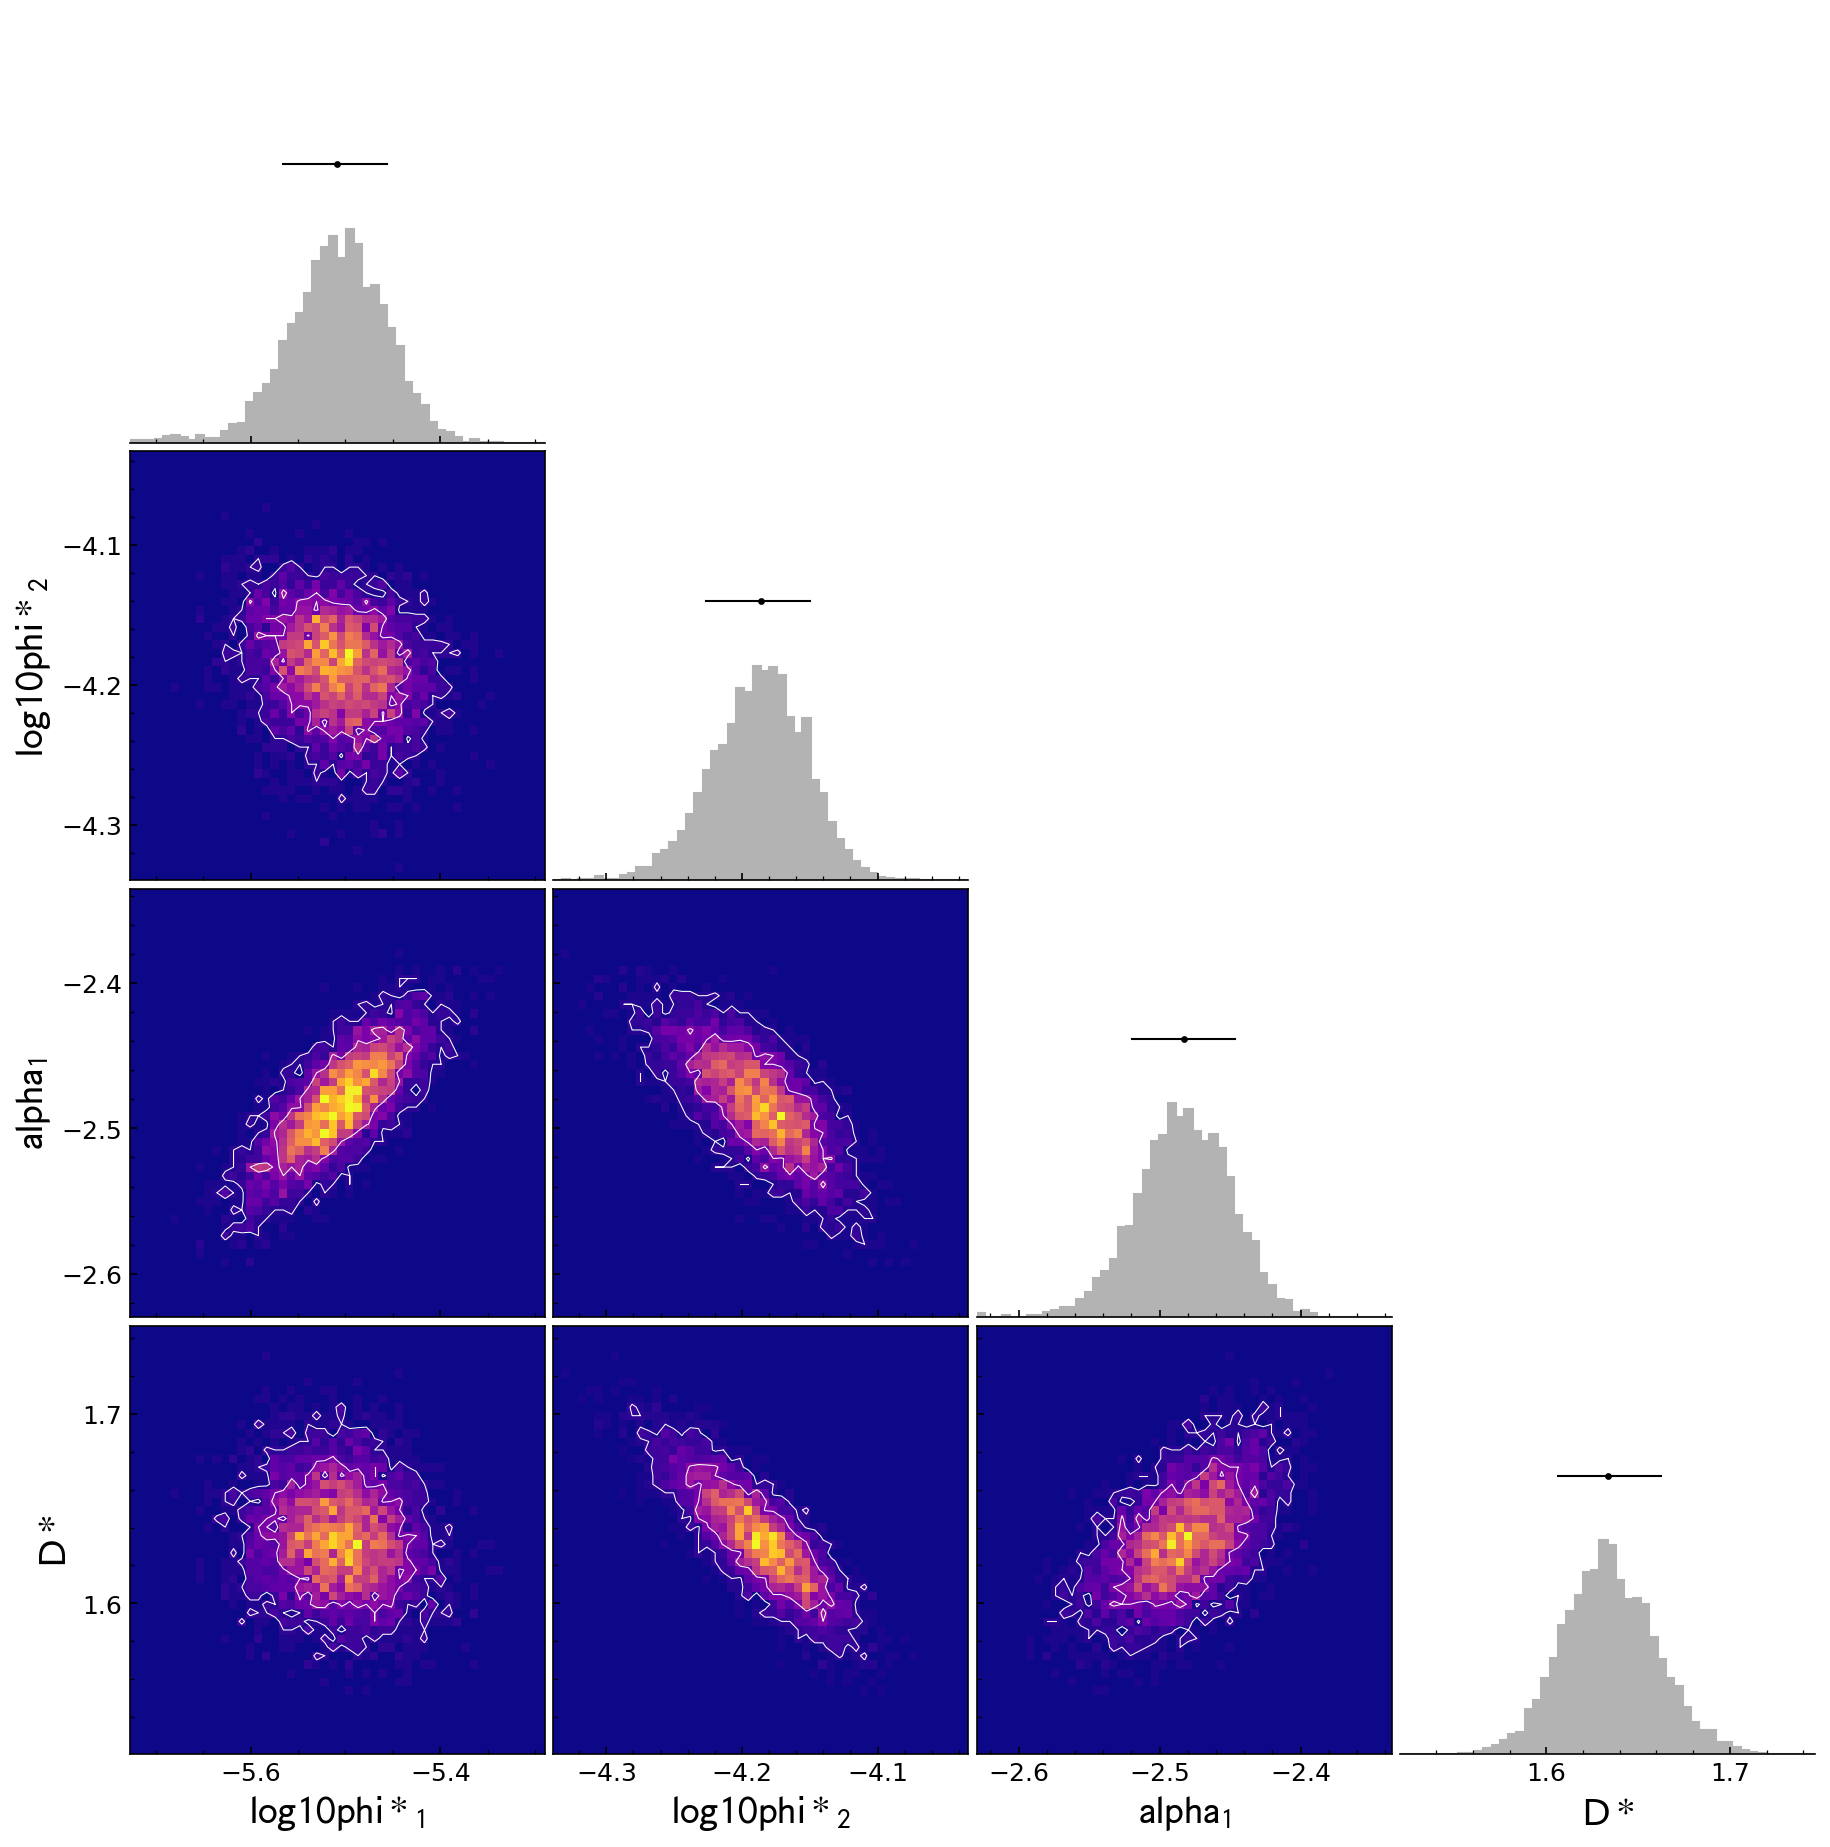
\includegraphics[width=0.8\textwidth]{images/posteriors_flares_7.png}
    \caption{Posteriors from the Galaxy Stellar Mass Function fit at $z = 7$. $\alpha_2$ is fixed at -1 and is not shown.
    }
    \label{fig:posteriors}
\end{figure*}


\begin{table*}
	\centering
	\begin{tabular}[t]{cccccc}
		\hline
		z &  M$^{*}$ & log$_{10}$($\phi^{*}_{1}$\,/(Mpc$^{-3}$ dex$^{-1}$)) & log$_{10}$($\phi^{*}_{2}$\,/(Mpc$^{-3}$ dex$^{-1}$)) & $\alpha_1$ \\
		\hline
		10 &            $9.117_{ - 0.045 }^{ +0.041 }$ &            $-6.557_{-0.197}^{+0.188 }$ &            $-4.871_{-0.07}^{+0.065 }$ &            $-3.542_{-0.206}^{+0.193}$ \\
		9 &            $9.488_{ - 0.044 }^{ +0.036 }$ &            $-6.372_{-0.112}^{+0.116 }$ &            $-4.832_{-0.057}^{+0.056 }$ &            $-3.07_{-0.077}^{+0.076}$ \\
		8 &            $9.577_{ - 0.041 }^{ +0.039 }$ &            $-5.904_{-0.08}^{+0.081 }$ &            $-4.565_{-0.058}^{+0.059 }$ &            $-2.83_{-0.048}^{+0.065}$ \\
		7 &            $9.831_{ - 0.035 }^{ +0.039 }$ &            $-5.443_{-0.054}^{+0.051 }$ &            $-4.374_{-0.059}^{+0.052 }$ &            $-2.515_{-0.032}^{+0.03}$ \\
		6 &            $10.089_{ - 0.035 }^{ +0.029 }$ &            $-5.057_{-0.047}^{+0.036 }$ &            $-4.156_{-0.046}^{+0.05 }$ &            $-2.293_{-0.023}^{+0.019}$ \\
		5 &            $10.326_{ - 0.02 }^{ +0.019 }$ &            $-4.686_{-0.024}^{+0.023 }$ &            $-3.942_{-0.034}^{+0.033 }$ &            $-2.11_{-0.011}^{+0.012}$ \\
		\hline
	\end{tabular}
	\caption{Best fitting double-Schechter function parameter values for the Galaxy Stellar Mass Function. $\alpha_{2}$ is fixed at $-1$.} \label{tab:schechter_params}
\end{table*}

\begin{table*}
	\centering
	\begin{tabular}[t]{cccccc}
		\hline
		z &  SFR$^{*}$ & log$_{10}$($\phi^{*}_{1}$\,/(Mpc$^{-3}$ dex$^{-1}$)) & log$_{10}$($\phi^{*}_{2}$\,/(Mpc$^{-3}$ dex$^{-1}$)) & $\alpha_1$ \\
		\hline
		5 &            $1.402_{ - 0.067 }^{ +0.049 }$ &            $-6.525_{-0.123}^{+0.142 }$ &            $-5.022_{-0.069}^{+0.07 }$ &            $-2.978_{-0.074}^{+0.071}$ \\
		5 &            $1.359_{ - 0.044 }^{ +0.036 }$ &            $-5.941_{-0.093}^{+0.093 }$ &            $-4.645_{-0.058}^{+0.058 }$ &            $-2.772_{-0.06}^{+0.064}$ \\
		5 &            $1.433_{ - 0.028 }^{ +0.032 }$ &            $-5.639_{-0.066}^{+0.059 }$ &            $-4.431_{-0.058}^{+0.049 }$ &            $-2.62_{-0.045}^{+0.051}$ \\
		5 &            $1.633_{ - 0.027 }^{ +0.03 }$ &            $-5.509_{-0.057}^{+0.052 }$ &            $-4.186_{-0.04}^{+0.036 }$ &            $-2.482_{-0.038}^{+0.036}$ \\
		5 &            $1.684_{ - 0.015 }^{ +0.015 }$ &            $-5.059_{-0.039}^{+0.041 }$ &            $-3.907_{-0.026}^{+0.024 }$ &            $-2.307_{-0.025}^{+0.026}$ \\
		5 &            $1.755_{ - 0.012 }^{ +0.011 }$ &            $-4.68_{-0.033}^{+0.033 }$ &            $-3.644_{-0.02}^{+0.02 }$ &            $-2.139_{-0.019}^{+0.02}$ \\
		\hline
	\end{tabular}
	\caption{Best fitting double-Schechter function parameter values for the Star Formation Rate distribution function. $\alpha_{2}$ is fixed at $-1$.}
	\label{tab:sfrf_schechter_params}
\end{table*}

\begin{table}
	\centering
	\begin{tabular}[t]{cccccc}
		\hline
		z & $x_{0} + 9.7$ & $\alpha_{1}$ & $\alpha_{2}$ & $\beta$ \\
		\hline
		5  & 9.60 & 1.23 & 0.62 & 1.42 \\
		6  & 9.45 & 1.27 & 0.70 & 1.60 \\
		7  & 9.35 & 1.31 & 0.72 & 1.76 \\
		8  & 9.20 & 1.33 & 0.80 & 1.90 \\
		9  & 9.16 & 1.31 & 0.91 & 1.93 \\
		10 & - & 1.24 & - & - \\
		\hline
	\end{tabular}
	\caption{Best fitting two-part piecewise-linear fits to the star-forming sequence.}
	\label{tab:sfs_params}
\end{table}


\section{The impact of cutting passive galaxies from the star forming sequence}
\label{sec:ssfr_cut}

\begin{figure}
	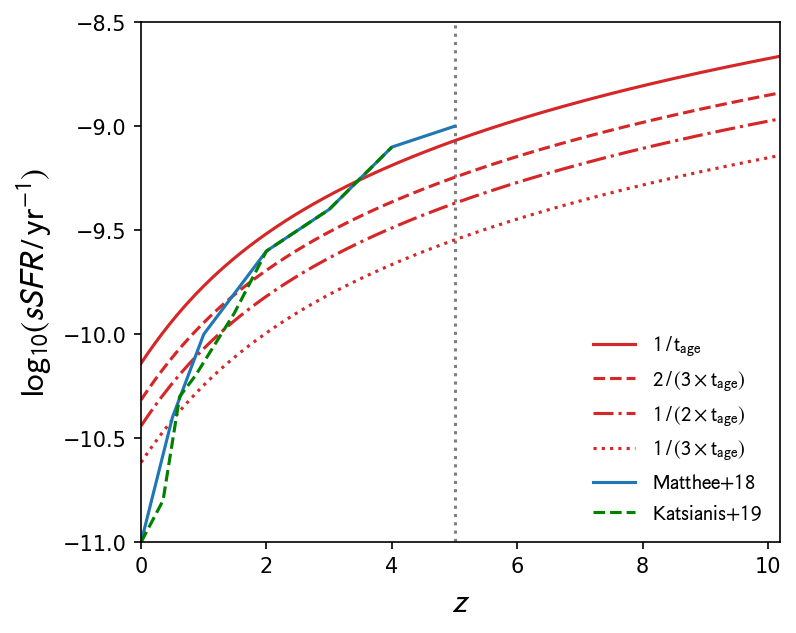
\includegraphics[width=\columnwidth]{images/ssfr_cut.png}
    \caption{Evolving sSFR cuts for passive galaxies. Cuts used in \protect\cite{katsianis_evolving_2019,matthee_origin_2019} shown for comparison.
    }
    \label{fig:ssfr_cut}
\end{figure}

In \sec{results:sfs} we showed the SFS assuming no cut for passive galaxies.
We now briefly explore the impact of applying an evolving cut in specific star formation rate (sSFR), and how this impacts the SFS.
We employ an sSFR cut that excludes those galaxies whose current star formation is insufficient to double the mass of the galaxy within twice the current age of the universe,
\begin{align}
\mathrm{sSFR} > \frac{1}{2 \times t_{\mathrm{age}}} \;\;,
\end{align}
which leads to an evolving threshold for quiescence with redshift, shown in \fig{ssfr_cut}.
Using this cut, we exclude 979 galaxies at $z = 5$ (out of a total of 32824 with stellar masses above $10^{8} \, M_{\odot}$).

\begin{figure}
	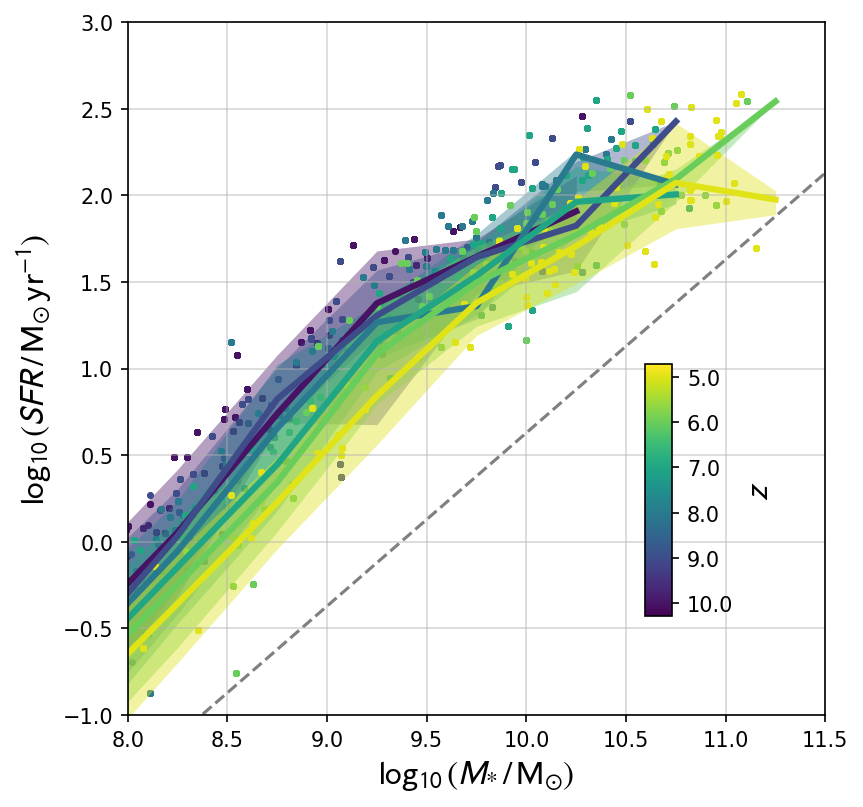
\includegraphics[width=\columnwidth]{images/sfs_all_cut.png}
    \caption{SFS assuming a sSFR cut for passive galaxies. This cut at $z = 5$ is shown by the dashed line. The relations are essentially identical to those without a passive galaxy cut.
    }
    \label{fig:sfs_all_cut}
\end{figure}

\fig{sfs_all_cut} shows the SFS assuming this cut.
There is alsmost no difference between this relation and that shown in \fig{sfs_all}.
We tested using different thresholds (mass multiples of $\times \frac{3}{2}$ and $\times 3$) and found that all our results are insensitive to the multiple of mass chosen.
Observations typically use UVJ colour to discriminate quiescent objects \citep[e.g.][]{whitaker_newfirm_2011}; at $z \sim 2$, this leads to a similar threshold for quiescence as a sSFR cut \citep{fang_demographics_2018}.
